\documentclass[11pt]{article}

\usepackage[margin=1in]{geometry}
\usepackage{amsmath,amssymb}
\usepackage{booktabs}
\usepackage{array}
\usepackage{xcolor}
\usepackage{tikz}
\usetikzlibrary{positioning}
\usepackage{enumitem}
\usepackage{hyperref}

\newcommand{\nb}{\textsc{nb}}
\newcommand{\bas}{\textsc{b}}
\newcommand{\slack}[1]{s_{#1}}

\title{Orbital Crossover with Bipartite Degenerate Matching:\\
a failing case on the $K_4$ fractional matching LP}
\author{EQLPSolver --- Orbital Crossover (branch \texttt{oc-bipartite-matching})}
\date{\today}

\begin{document}
\maketitle

\begin{abstract}
This note documents a concrete instance on which the current implementation of
the bipartite degenerate-matching pass (\texttt{matchDegenerateResiduals}) fails.
The instance is the fractional matching LP of the complete graph $K_4$. We give
the instance, its coarsest equitable partition, the lifted (extended) basis, a
step-by-step account of what \emph{baseline} orbital crossover (OC) does, and a
step-by-step account of what the \emph{matching} variant does --- including the
HiGHS-level failure. The root cause is that the matched starting basis is
\textbf{singular} (its $9\times9$ basis matrix has rank $8$); HiGHS cannot factor
it, patches the rank deficiency with a logical column, lands primal-infeasible,
and returns a final model status of \texttt{Unknown}. This singularity has been
confirmed three ways: by hand, by an independent exact ($\mathbb{Q}$-arithmetic)
rank/null-space computation, and by a dense rank check built into HiGHS itself
(\texttt{ocVerifyBasisSingularity} in \texttt{Highs.cpp}) that runs on the actual
in-solver basis. The purpose is to localise the problem so the algorithm or its
implementation can be corrected.
\end{abstract}

\section{The instance}

The variables are the six edges of $K_4$; the constraints are the four vertices,
each requiring that the edges incident to it sum to at most one (the fractional
matching polytope). With the indexing
\[
x_1=(1,2),\quad x_2=(1,3),\quad x_3=(1,4),\quad
x_4=(2,3),\quad x_5=(2,4),\quad x_6=(3,4),
\]
the LP is
\[
\begin{aligned}
\max\quad & x_1+x_2+x_3+x_4+x_5+x_6\\
\text{s.t.}\quad
c_1:\;& x_1+x_2+x_3 \le 1\\
c_2:\;& x_1+x_4+x_5 \le 1\\
c_3:\;& x_2+x_4+x_6 \le 1\\
c_4:\;& x_3+x_5+x_6 \le 1\\
& 0\le x_i\le 1,\quad i=1,\dots,6.
\end{aligned}
\]
There are \textbf{six variables and four constraints}, so a basic feasible
solution has at most four nonzero structural variables: not all variables can be
basic at once. The incidence matrix $A$ (rows = vertices, columns = edges) is
\[
A=
\begin{array}{c|cccccc}
       & x_1 & x_2 & x_3 & x_4 & x_5 & x_6\\\hline
c_1\;(v_1) & 1 & 1 & 1 & 0 & 0 & 0\\
c_2\;(v_2) & 1 & 0 & 0 & 1 & 1 & 0\\
c_3\;(v_3) & 0 & 1 & 0 & 1 & 0 & 1\\
c_4\;(v_4) & 0 & 0 & 1 & 0 & 1 & 1
\end{array}
\]
Every column sums to $2$ (each edge has two endpoints) and every row sums to $3$
($K_4$ is $3$-regular). The optimal value is $2$, attained at any perfect
matching, e.g. $x_1=x_6=1$ (edges $(1,2)$ and $(3,4)$), all other $x_i=0$.

\section{Coarsest equitable partition}

Because the data are uniform (all objective coefficients $1$, all right-hand
sides $1$, all bounds $[0,1]$, all senses $\le$) and the bipartite
variable/constraint incidence is biregular (constant column sum $2$, constant row
sum $3$), the \emph{trivial} partition
\[
V=\{x_1,\dots,x_6\}\ \text{(one cell)},\qquad
C=\{c_1,\dots,c_4\}\ \text{(one cell)}
\]
is equitable, and being minimal it is the coarsest equitable partition. One
refinement round leaves it unchanged: every edge sees exactly two same-coloured
vertices, every vertex sees exactly three same-coloured edges. Thus the initial
aggregate LP (ALP) has a single column $x$ and a single constraint:
\[
\max\;6x \quad\text{s.t.}\quad 3x\le 1,\qquad x=\tfrac13,\quad \text{objective }2 .
\]
In the ALP solve $x$ is \emph{basic} and the single (aggregated) constraint is
binding, so its slack is \emph{nonbasic}.

\section{The extended LP and the lifted basis}

Because the refinement threshold is not reached on such a small instance, the
solver lifts directly from the coarsest partition to the discrete partition in a
single step. The extended LP (ELP/EALP) at that lift has
\begin{itemize}[nosep]
  \item \textbf{11 columns}: the six structural variables $x_1,\dots,x_6$ and
  five residual (linking) variables $r_{i,1}=x_i-x_1$ for $i=2,\dots,6$;
  \item \textbf{9 rows}: the four original vertex constraints $c_1,\dots,c_4$ and
  five linking rows (one per residual).
\end{itemize}
A basis therefore has $9$ basic variables. The lifted basis produced by
\texttt{buildColBasis}/\texttt{buildRowBasis}, \emph{before} any matching and
\emph{before} any residual pivots, is shown in Table~\ref{tab:lifted}.

\begin{table}[h]
\centering
\begin{tabular}{lll}
\toprule
variable & status & value\\
\midrule
$x_1,x_2,x_3,x_4,x_5,x_6$ & \bas\ (basic) & $\tfrac13$ each\\
$\slack{c_1}$ (representative constraint) & \nb\ (lower) & $0$ (binding)\\
$\slack{c_2},\slack{c_3},\slack{c_4}$ (sibling constraints) & \bas\ (basic) & $0$ (degenerate)\\
$r_{2,1},r_{3,1},r_{4,1},r_{5,1},r_{6,1}$ & \nb\ (lower) & $0$\\
linking-row slacks $L_1,\dots,L_5$ & \nb\ (lower) & $0$\\
\bottomrule
\end{tabular}
\caption{Lifted basis before matching and before residual pivots. Basic count
$=6\ \text{structural}+3\ \text{slacks}=9=\text{num\_row}$.}
\label{tab:lifted}
\end{table}

\paragraph{Reasons for the statuses.}
\begin{itemize}[nosep]
  \item Every $x_i$ inherits the status of its parent aggregate column, which was
  basic ($x=\tfrac13$); hence all six edges are basic.
  \item $c_1$ is the representative constraint, so its slack inherits the
  aggregate slack's nonbasic status.
  \item $c_2,c_3,c_4$ are newly created sibling rows and are left basic by the
  default fill in \texttt{buildRowBasis}.
  \item The residual columns are parked nonbasic at their lower bound; these are
  the variables OC normally pivots in.
\end{itemize}
This lifted point is feasible but \textbf{degenerate}: all four vertex
constraints are tight at the all-$\tfrac13$ point ($3\cdot\tfrac13=1$), so the
three basic slacks $\slack{c_2},\slack{c_3},\slack{c_4}$ sit at value $0$.

\section{Baseline orbital crossover (no matching)}

\subsection*{Step by step}
\begin{enumerate}[nosep]
  \item Solve the ALP: $x=\tfrac13$, objective $2$.
  \item Lift to the EALP, producing the basis of Table~\ref{tab:lifted}
        (5 residuals nonbasic).
  \item Run the OC primal phase, which pivots the residual columns into the basis
        one at a time (highest index first). Five residuals $\Rightarrow$ five
        pivots. Each residual pivot ejects one currently-basic variable.
  \item When all residuals are basic, truncate them to obtain an optimal basic
        feasible solution of the original LP.
\end{enumerate}

\subsection*{HiGHS log (trimmed)}
\begin{verbatim}
Solving LP with Orbital Crossover
Using Orbital Crossover
  Iteration        Objective     Infeasibilities num(sum)
          1     2.0000000000e+00 Pr: 0(0) 0s
          6     2.0000000000e+00 Pr: 0(0) 0s
Model   status      : Optimal
Objective value     :  2.0000000000e+00
\end{verbatim}
The OC phase runs from iteration $1$ to $6$: exactly \textbf{five residual
pivots}, ending \texttt{Optimal}.

\subsection*{Final basis}
The basis HiGHS reports for the EALP is (status codes
$1=$ basic, $0=$ nonbasic-lower, $2=$ nonbasic-upper):
\begin{verbatim}
# Columns (11):  1 0 0 1 1 1 1 1 1 1 1
# Rows (9):      2 2 2 2 0 0 0 0 0
\end{verbatim}
Decoded in Table~\ref{tab:basefinal}.

\begin{table}[h]
\centering
\begin{tabular}{lll}
\toprule
variable & status & value\\
\midrule
$x_1$ & \bas & $1$\\
$x_2,x_3$ & \nb\ (lower) & $0$\\
$x_4,x_5$ & \bas & $0$ (degenerate)\\
$x_6$ & \bas & $1$\\
$r_{2,1},\dots,r_{6,1}$ (all five residuals) & \bas & ---\\
$\slack{c_1},\slack{c_2},\slack{c_3},\slack{c_4}$ & \nb\ (upper) & $0$ (tight)\\
linking-row slacks $L_1,\dots,L_5$ & \nb\ (lower) & $0$\\
\bottomrule
\end{tabular}
\caption{Final EALP basis after baseline OC. Basic count
$=4\ \text{structural}+5\ \text{residuals}=9$.}
\label{tab:basefinal}
\end{table}

\paragraph{Interpretation.}
The vertex is the perfect matching $x_1=x_6=1$, all other $x_i=0$, objective $2$
(dual $0.5$ on each vertex constraint). All five residuals are basic, so they
truncate cleanly, leaving the original-LP basis $\{x_1,x_4,x_5,x_6\}$ with
$x_2,x_3$ nonbasic and all four constraint slacks nonbasic. The vertex is itself
degenerate: $x_4,x_5$ are basic at value $0$.

\paragraph{Key observation.}
Reaching this vertex required the five residual pivots to eject \emph{two
structural variables} ($x_2,x_3$) in addition to the three basic slacks
($\slack{c_2},\slack{c_3},\slack{c_4}$): $2+3=5$ leaving variables for the five
entering residuals. This observation matters in the next section.

\section{Matching variant (\texttt{oc\_match\_degenerate = true})}

The matching pass runs after \texttt{buildBasis} and tries to place residuals
into the basis combinatorially (a maximum bipartite matching), so they need not
be pivoted in by the simplex.

\subsection*{The bipartite graph the code builds}

\paragraph{Right nodes (residuals).}
$r_{2,1},r_{3,1},r_{4,1},r_{5,1},r_{6,1}$ --- one per child edge, all linked to
the representative edge $x_1$.

\paragraph{Left nodes (candidate swap targets).}
The code admits three kinds of left node: degenerate structural columns (basic
\emph{and} at a bound), degenerate slacks (basic with zero dual), and children of
nonbasic slacks; in every case the candidate must currently be \emph{basic}
(only a basic variable can be swapped out). For this instance:
\begin{itemize}[nosep]
  \item \emph{Degenerate structural columns:} \textbf{none}. Every edge is at
        $\tfrac13$, strictly interior to $[0,1]$.
  \item \emph{Degenerate slacks:} \textbf{none}. The aggregate slack is nonbasic.
  \item \emph{Children of the nonbasic slack:} the aggregate slack is nonbasic,
        so all four vertex slacks are its children. The representative child
        $\slack{c_1}$ inherited \emph{nonbasic} status and is excluded by the
        basic-only guard. The remaining three, $\slack{c_2},\slack{c_3},
        \slack{c_4}$, are basic and become the left nodes.
\end{itemize}
So the left set is $\{\slack{c_2},\slack{c_3},\slack{c_4}\}$ --- only three nodes
against five residuals.

\paragraph{Edges.}
A slack $\slack{c_v}$ is joined to residual $r_{i,1}$ iff edges $x_i$ and $x_1$
have \emph{different} coefficients in constraint $v$, i.e. $A[v,x_i]\ne
A[v,x_1]$ --- equivalently, exactly one of edges $i$ and $1=(1,2)$ touches vertex
$v$. (Rationale: then perturbing $r_{i,1}$ changes the activity of constraint
$v$, forcing its basic slack to move --- a degenerate pivot.) Using $A$:
\[
\begin{aligned}
\slack{c_2}\ (v_2,\ A[v_2,x_1]=1):&\quad r_{2,1},\,r_{3,1},\,r_{6,1}\\
\slack{c_3}\ (v_3,\ A[v_3,x_1]=0):&\quad r_{2,1},\,r_{4,1},\,r_{6,1}\\
\slack{c_4}\ (v_4,\ A[v_4,x_1]=0):&\quad r_{3,1},\,r_{5,1},\,r_{6,1}
\end{aligned}
\]

\begin{figure}[h]
\centering
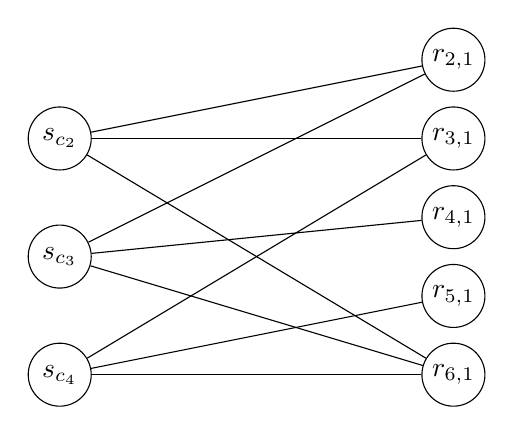
\begin{tikzpicture}[every node/.style={draw,circle,minimum size=8mm,inner sep=1pt},
                    >=stealth, node distance=10mm]
  % left nodes
  \node (s2) at (0,3) {$\slack{c_2}$};
  \node (s3) at (0,1.5) {$\slack{c_3}$};
  \node (s4) at (0,0) {$\slack{c_4}$};
  % right nodes
  \node (r2) at (5,4) {$r_{2,1}$};
  \node (r3) at (5,3) {$r_{3,1}$};
  \node (r4) at (5,2) {$r_{4,1}$};
  \node (r5) at (5,1) {$r_{5,1}$};
  \node (r6) at (5,0) {$r_{6,1}$};
  % edges
  \draw (s2)--(r2); \draw (s2)--(r3); \draw (s2)--(r6);
  \draw (s3)--(r2); \draw (s3)--(r4); \draw (s3)--(r6);
  \draw (s4)--(r3); \draw (s4)--(r5); \draw (s4)--(r6);
\end{tikzpicture}
\caption{The bipartite graph built for $K_4$. Left: the three basic slacks
(children of the nonbasic aggregate slack). Right: the five residuals. There are
no structural left nodes because no edge is at a bound.}
\label{fig:bip}
\end{figure}

\subsection*{Maximum matching}
With only three left nodes, the matching saturates at most three of the five
residuals, e.g.
\[
\slack{c_2}\!-\!r_{2,1},\qquad \slack{c_3}\!-\!r_{4,1},\qquad
\slack{c_4}\!-\!r_{3,1},
\]
leaving $r_{5,1}$ and $r_{6,1}$ unmatched. The pass therefore applies three
swaps: for each matched pair it sets the residual basic and its matched slack
nonbasic.

\subsection*{What goes wrong in HiGHS}

\begin{verbatim}
Solving LP with Orbital Crossover
Using Orbital Crossover
  Iteration        Objective     Infeasibilities num(sum)
          1     2.0000000000e+00 Pr: 2(2); Du: 1(6) 0s   <-- INFEASIBLE start
          4     2.0000000000e+00 Pr: 0(0) 0s
Model   status      : Unknown
Objective value     :  2.0000000000e+00
\end{verbatim}

After the three swaps are applied, the basis handed to the OC simplex is
\textbf{singular}, and only then \emph{primal infeasible}. The log reports
\texttt{Pr: 2(2)} (two infeasible variables, total infeasibility $2$) at the very
first iteration of the OC phase. The simplex performs a few recovery pivots and
recovers the objective value $2.0$, but it cannot certify optimality from this
corrupted basis, so the final model status is \texttt{Unknown} (and the process
returns a nonzero exit code). Baseline, in contrast, starts from a nonsingular,
feasible basis and ends \texttt{Optimal}.

\paragraph{The starting basis (as actually built).}
With residual indexing $r_{2,1},\dots,r_{6,1}$ and the matcher iterating the
three left slacks in row order, Kuhn's algorithm saturates all three slacks and
leaves $r_{5,1},r_{6,1}$ unmatched (the precise pairing
$r_{2,1}\!-\!\slack{c_2}$, $r_{3,1}\!-\!\slack{c_4}$, $r_{4,1}\!-\!\slack{c_3}$
differs from the ``e.g.'' above but yields the \emph{same} basis). The status
vector handed to HiGHS is, with codes $1=$ basic, $0=$ nonbasic-lower,
\[
\begin{aligned}
\text{Columns (11): }& x_1\,x_2\,x_3\,x_4\,x_5\,x_6 \mid r_{2,1}\,r_{3,1}\,r_{4,1}\,r_{5,1}\,r_{6,1}
   \;=\; 1\,1\,1\,1\,1\,1 \mid 1\,1\,1\,0\,0\\
\text{Rows (9): }& \slack{c_1}\,\slack{c_2}\,\slack{c_3}\,\slack{c_4} \mid L_1\dots L_5
   \;=\; 0\,0\,0\,0 \mid 0\,0\,0\,0\,0 .
\end{aligned}
\]
The basic set is the six edges and the three matched residuals: $6+3=9$ basic
variables and \emph{zero} basic slacks. The cardinality is therefore correct
($9 = \text{num\_row}$); the defect is rank, not count.

\paragraph{Singularity of the basis matrix.}
Ordering the basic columns $x_1,\dots,x_6,r_{2,1},r_{3,1},r_{4,1}$ and the rows
$c_1,\dots,c_4,L_2,\dots,L_6$, the $9\times9$ basis matrix is
\[
B=
\begin{pmatrix}
1&1&1&0&0&0& 0&0&0\\
1&0&0&1&1&0& 0&0&0\\
0&1&0&1&0&1& 0&0&0\\
0&0&1&0&1&1& 0&0&0\\
-1&1&0&0&0&0& -1&0&0\\
-1&0&1&0&0&0& 0&-1&0\\
-1&0&0&1&0&0& 0&0&-1\\
-1&0&0&0&1&0& 0&0&0\\
-1&0&0&0&0&1& 0&0&0
\end{pmatrix}.
\]
Exact rational elimination gives $\det B = 0$, $\operatorname{rank} B = 8$, and a
one-dimensional null space spanned by
\[
v=\bigl(-\tfrac13,-\tfrac13,\tfrac23,\tfrac23,-\tfrac13,-\tfrac13,\;0,\;1,\;1\bigr)
\quad(\text{over } x_1,\dots,x_6,r_{2,1},r_{3,1},r_{4,1}),\qquad Bv=0 .
\]
The mechanism: swapping out all three slacks $\slack{c_2},\slack{c_3},\slack{c_4}$
(with $\slack{c_1}$ already nonbasic) forces all four vertex rows to equality, but
each edge meets exactly two vertices, so the four vertex rows sum to
$2\,(x_1+\dots+x_6)$ --- a dependency that, together with $r_{5,1},r_{6,1}$ held
nonbasic, costs one unit of rank.

\paragraph{Runtime confirmation inside HiGHS.}
A dense rank check (\texttt{ocVerifyBasisSingularity}, called after
\texttt{setBasis} in the orbital-crossover loop and gated on
\texttt{oc\_match\_degenerate}) rebuilds $B$ from the live \texttt{ealp\_} and
\texttt{ealpBasis\_} and factors it independently of HiGHS's own LU. On this
instance it prints
\begin{verbatim}
[OC-VERIFY after-match] num_row=9  basic: struct=9 slack=0 total=9 (cardinality OK)
[OC-VERIFY after-match] dense rank(B)=8 of 9  deficiency=1  min|pivot|=1.000e+00
                        ==> B IS SINGULAR (not invertible)
\end{verbatim}
The clean pivot magnitude (\texttt{min|pivot|=1.000e+00}) shows this is a
structural rank deficiency, not numerical noise.

\subsection*{Why it fails (diagnosis)}

The bipartite graph itself appears faithful to the design: right nodes are the
remaining residuals, left nodes are the degenerate variables / children of
nonbasic slacks, and the edge rule is the ``different coefficient in that
constraint'' condition. The failure is in \emph{applying} the matched swaps, for
two compounding reasons specific to this instance.

\begin{enumerate}[label=(\roman*)]
  \item \textbf{The matching cannot eject the structural variables the vertex
  needs.} As noted in the baseline analysis, the optimal vertex is reached only
  by ejecting the structural variables $x_2,x_3$ from the basis. But no edge is
  at a bound, so there are \emph{no} degenerate structural left nodes; the only
  swap targets are slacks. The matching has no mechanism to move $x_2,x_3$ out,
  so the combinatorial swaps can never reproduce the baseline vertex.

  \item \textbf{The matched ``pivots'' are not mutually independent, so applying
  them simultaneously is not the same as performing them sequentially, and the
  result is a singular basis.} All five residuals share the same parent $x_1$ and
  act through overlapping basic structural variables. A maximum matching
  guarantees only that each residual is paired with a \emph{distinct} slack; it
  does \emph{not} guarantee that the resulting basis columns are linearly
  independent. Flipping all three statuses together yields the rank-$8$ matrix
  $B$ above ($\det B = 0$): the basis is singular before feasibility is even at
  issue. HiGHS cannot factor it, patches the rank deficiency with a logical
  column, and only then reports the primal infeasibility \texttt{Pr: 2(2)}.
\end{enumerate}

In short, on this instance the maximum matching produces a set of status flips
that does \emph{not} correspond to a valid simultaneous sequence of degenerate
pivots, and the resulting starting basis is \textbf{singular} (rank $8$ of $9$),
hence not a basis at all. This is consistent with the matching scheme being, as
noted in its source, a conjectured construction whose proof has not been
completed.

\section{Summary}

\begin{itemize}[nosep]
  \item Baseline OC: lifts to a feasible degenerate basis, performs five residual
  pivots (ejecting slacks $\slack{c_2},\slack{c_3},\slack{c_4}$ and structural
  $x_2,x_3$), and terminates \texttt{Optimal} at the perfect-matching vertex.
  \item Matching OC: builds a faithful bipartite graph but, lacking any
  degenerate structural left node, can only swap residuals against three slacks;
  the maximum matching of size three, applied simultaneously, yields a
  \textbf{singular} starting basis (rank $8$ of $9$, $\det B = 0$, cardinality
  correct at $9$). HiGHS cannot factor it, so it is primal-infeasible after a
  logical patch and ends with status \texttt{Unknown}. Verified by hand, by exact
  rational computation, and by the in-solver check \texttt{ocVerifyBasisSingularity}.
  \item Likely fixes to investigate: (a) verify each matched swap individually
  preserves feasibility / nonsingularity before committing it; (b) treat the
  matched swaps as a \emph{sequence} of degenerate pivots rather than a
  simultaneous status flip; (c) reconsider whether structural variables must be
  admissible swap targets when the vertex requires ejecting them.
\end{itemize}

\section{Toward a fix: a nonsingular combinatorial matching}

This section develops an algorithm that chooses which residuals (right nodes) to
swap against which basic variables (left nodes) so that the resulting starting
basis is \emph{guaranteed} nonsingular, using only combinatorial tests --- no LU
factorization and no trial (``fake'') pivots. It works at \emph{any} lift, from
partition $i$ to partition $j$ (which need not be discrete): the blocks below are
defined by the current partition pair and the current aggregate matrix.

\subsection{Two independent guards}

The original left-node rule (``basic \emph{and} at a bound'') is a
\textbf{feasibility} rule: a value-preserving degenerate swap keeps the solution
in bounds. It says nothing about \textbf{nonsingularity}, which is why $K_4$
failed. The fix keeps that rule for feasibility and adds a \emph{separate}
nonsingularity oracle:
\begin{enumerate}[nosep,label=(\roman*)]
  \item \textbf{Feasibility guard} (unchanged): left nodes are value-preserving
  basic variables (degenerate structural columns, degenerate slacks, children of
  nonbasic slacks).
  \item \textbf{Nonsingularity guard} (new): accept a matched edge only if an
  oracle certifies the basis stays nonsingular. Process edges greedily
  (Kruskal-style); reject-and-continue on conflict.
\end{enumerate}

\subsection{The unit-column reduction}

Every residual column is a \textbf{unit vector}: $r_{i,j}=x_i-x_j$ contributes a
single $-1$, in its own linking row, and nowhere else. Hence assigning a basic
residual to its linking row is a unit-column cofactor expansion, and
\[
\det(\text{full basis}) \;=\; \pm\,\det\bigl(\text{basis with every basic
residual's column \emph{and} its linking row deleted}\bigr).
\]
So residuals and their linking rows drop out of the determinant. What remains is
a square submatrix of the \emph{original} constraint matrix $A$: the basic
structural columns against the surviving rows (tight constraints plus the linking
rows of \emph{uncut} residuals). \textbf{The matching's only job is to keep that
$A$-submatrix nonsingular.} (Verified on $K_4$: the full $9\times9$ basis and the
reduced $6\times6$ $A$-submatrix have the same deficiency $1$.)

A consequence we use throughout: because all residuals here share the parent
$x_1$, an \emph{uncut} residual $r_{i,1}$ ties $x_i$ to $x_1$ (they are forced
equal), while a \emph{cut} (placed-basic) residual decouples $x_i$. Cutting a
residual removes its linking row from the reduced matrix.

\subsection{What is decidable combinatorially, and what is not}

The reduced problem is linear independence of columns of $A$. In general this is
\emph{not} a graphic matroid, so it has no factorization-free oracle (see the
main analysis). Two regimes are usable:
\begin{itemize}[nosep]
  \item \textbf{Uniform blocks} (all nonzeros in the orbit block equal --- always
  true for $0/1$ matrices, i.e.\ OC's combinatorial target): singularity is a
  pure pattern property (scale-invariant), so a parity/even-cycle test applies.
  \item \textbf{Non-uniform blocks}: singularity depends on the actual values;
  only a conservative structural test is safe.
\end{itemize}

\subsection{Oracle A --- conservative, provably safe for any LP}

\textbf{Rule.} Accept a set of swaps only if the bipartite sparsity graph of the
reduced matrix (rows $\times$ basic columns) stays a \emph{forest} that admits a
perfect matching.

\textbf{Why it is correct.} A square matrix whose bipartite sparsity graph is a
forest has a \emph{unique} transversal, hence is permutable to triangular, hence
nonsingular for \emph{any} nonzero coefficient values. No cancellation is
possible. This is a theorem, independent of the LP.

\begin{verbatim}
UNION-FIND over {row nodes} U {column nodes}, initially all singletons.
for each candidate swap (slack c_v <- residual r_i), in greedy order:
    tentatively form the reduced matrix rows/cols after this swap
    ok = true
    for each nonzero (row R, col C) introduced or retained:
        if find(R) == find(C): ok = false; break     # would close a cycle
        else union(R, C)
    if ok and a perfect matching still exists: accept; else: reject (roll back)
\end{verbatim}

\textbf{Cost.} $O(\text{nnz}\cdot\alpha(n))$. No linear algebra.

\textbf{$K_4$ example.} Every candidate swap makes some vertex constraint tight,
and each vertex row shares columns with the linking rows already present, closing
a cycle immediately. Oracle A therefore \textbf{places $0$ residuals} and safely
degrades to baseline OC (five simplex pivots, \texttt{Optimal}). Safe, but weak
on this dense instance --- validated: $0$ false accepts over all $46$ candidate
$K_4$ matchings.

\subsection{Oracle B --- parity/even-cycle, exact for uniform blocks (full-tight
regime)}

For a $0/1$ orbit block, form the \textbf{constraint graph} $G$: nodes are the
constraints of the cell, and each structural variable $x_e$ is an edge joining the
two constraints it appears in. For $K_4$, $G=K_4$:
\[
x_1{=}(c_1,c_2),\ x_2{=}(c_1,c_3),\ x_3{=}(c_1,c_4),\
x_4{=}(c_2,c_3),\ x_5{=}(c_2,c_4),\ x_6{=}(c_3,c_4).
\]
A linear dependency among the tight constraint rows corresponds to a signing
$\varepsilon\in\{\pm1\}$ of the (tight) constraint nodes: an edge with endpoints
of opposite sign cancels; an edge within one side survives. The reduced basis is
\emph{singular} iff there is a nonzero signing under which (a) every \emph{cut}
edge cancels and (b) the surviving (uncut) contributions balance to zero --- an
\textbf{even cycle} in the parity sense. This is detected by a parity union-find
(2-coloring) plus a signed-degree balance, with no rank computation.

\textbf{$K_4$ example, step by step.} Left nodes are the three basic slacks
$\slack{c_2},\slack{c_3},\slack{c_4}$ ($\slack{c_1}$ is already nonbasic). Their
adjacency (residual differs from parent in that constraint):
\[
\slack{c_2}:\{r_2,r_3,r_6\},\quad \slack{c_3}:\{r_2,r_4,r_6\},\quad
\slack{c_4}:\{r_3,r_5,r_6\}.
\]
Greedy with the parity oracle:
\begin{center}
\begin{tabular}{lll}
\toprule
step & decision & reason\\
\midrule
$\slack{c_2}\leftarrow r_2$ & \textbf{accept} & no cycle yet\\
$\slack{c_3}\leftarrow r_4$ & \textbf{accept} & still nonsingular\\
$\slack{c_4}\leftarrow r_3$ & reject & all four tight, $L_6$ present: even cycle $c_1{+}c_2{-}c_3{-}c_4{+}2L_6{=}0$\\
$\slack{c_4}\leftarrow r_5$ & reject & same dependency ($L_6$ still present)\\
$\slack{c_4}\leftarrow r_6$ & \textbf{accept} & cutting $r_6$ deletes $L_6$; cycle broken\\
\bottomrule
\end{tabular}
\end{center}
Final matching $\{\slack{c_2}{\leftarrow}r_2,\ \slack{c_3}{\leftarrow}r_4,\
\slack{c_4}{\leftarrow}r_6\}$. The reduced basis is $6\times6$ of rank $6$
(\textbf{nonsingular}, rank-verified). The key move: same coverage as the buggy
matching (three residuals), but the cut set is chosen to break the even cycle by
cutting $r_6$ (deleting the offending $L_6$) instead of leaving $r_5,r_6$ uncut.

\textbf{Net effect on $K_4$.} Three residuals placed combinatorially, leaving
$r_3,r_5$ for the simplex ($\approx2$ pivots to eject the structural $x_2,x_3$)
--- three pivots saved versus baseline, and no \texttt{Unknown}. All three swaps
are value-preserving, so the starting basis is feasible.

\textbf{Scope and honest limitation.} Oracle B is exact when all constraints of
the cell are tight (the full-lift regime, where $K_4$'s decisive case lives). For
\emph{partial} matchings (only some constraints tight) no simple combinatorial
invariant tested matches the true rank --- unique-transversal agreed on $15/46$
$K_4$ matchings, transversal parity and $\mathrm{GF}(2)$-nonsingularity on
$40/46$, and the hand-derived signing criterion had $4$ false accepts. So Oracle
B is \emph{not} unconditionally safe as stated; it must either be restricted to
the full-tight regime, or paired with the in-solver check
\texttt{ocVerifyBasisSingularity} as a guard that falls back to Oracle A (or to
plain simplex pivots) whenever it would emit a singular basis.

\subsection{Recommended composition}

\begin{enumerate}[nosep]
  \item Apply the feasibility guard to fix the left-node set.
  \item If the block is uniform \emph{and} in the full-tight regime, run Oracle B
  (maximal safe placement).
  \item Otherwise run Oracle A (always safe, possibly fewer placements).
  \item In all cases, gate the emitted basis through
  \texttt{ocVerifyBasisSingularity}; on a singular verdict, drop the last
  accepted swaps until nonsingular. Residuals not placed are left nonbasic for
  the simplex (the CHUZC skip-guard already handles them). The result is never
  worse than baseline OC and never emits a singular basis.
\end{enumerate}

A runnable prototype of both oracles, the greedy, and the exhaustive validation
against exact rank lives in \texttt{docs/matching\_oracle\_prototype.py}.

\end{document}
